% This file provides a template to format JASSS articles v.0.5, 2015-03-24

% In order to be compiled, the following packages should be installed in your system:
% graphicx,xcolor, booktabs,amsmath, ifthen, geometry, authblk, natbib, endnotes

 % Please use pdflatex

% The font used is Source Sans Pro, normally included in Tex Live and other  major LaTeX distributions
% Location at CTAN: http://www.ctan.org/tex-archive/fonts/sourcesanspro/
% See also: http://www.tug.dk/FontCatalogue/sourcesanspro/

%%%%%%%%%%%%%%%%%%%%%%%%%%%%%%%%%%%%%%%%%%%%%%

\documentclass{JASSS}

%%%%%%%%%%%%%%%%%%%%%%%%%%%%%%%%%%%%%%%%%%%%%%

% Editorial fields (to be set in case of publication)
% Please leave this section untouched
%\doinum{10.18564/jasss.xxxx}
%\volume{xx}
%\issue{x}
%\article{x}
%\pubyear{20xx}
%\received{dd-mmm-yyyy}
%\accepted{dd-mmm-yyyy}
%\published{dd-mmm-yyyy}

%%%%%%%%%%%%%%%%%%%%%%%%%%%%%%%%%%%%%%%%%%%%%%

% title, authors and affiliations

\title{Crime prevention via gun laws: An emotion driven approach}

%All authors should be included in the submission. To anonymise the submission, set to 'true' the \reviewcopy command below. However, before submitting  you can check that all the informations you entered are correct by temporarily setting it to 'false'. Please remember to set it back to 'true' before the submission.
\reviewcopy{false}

%\author[1]{Tierry H\"ormann}
%\affil[1]{ETH Z\"urich}

% Subsequent author should be included using the following template. You can add more in case of need, just remember to appropriately set the corresponding number.  Please check the the authblk package documentation  in case of doubts

%\author[2]{}
%\affil[2]{}

%\author[3]{Third author here}
%\affil[3]{Affiliation of the third author here}

%\author[4]{fourth author here}
%\affil[4]{fourth of the third author here}

% In case of multiple affiliation for the same author:

%\author[1,2]{Author name here}
%\affil[1]{First affiliation}
%\affil[2]{Second affiliation}

%  In case of several authors sharing the same affiliation:

\author[1]{Tierry H\"ormann}
\author[1]{Timo Laudi}
\affil[1]{ETH Z\"urich, Switzerland}

% email for the corresponding author
\email{tierryh@student.ethz.ch}

%%%%%%%%%%%%%%%%%%%%%%%%%%%%%%%%%%%%%%%%%%%%%%

% NOTES. Please use endnotes. Notes should be placed after the main text and appendices and before the references. Also remember to uncomment the \theendnotes commands at the end of the document (just before the references)

%%%%%%%%%%%%%%%%%%%%%%%%%%%%%%%%%%%%%%%%%%%%%%

% REFERENCES should be included using the \citep, \citet, etc. commands provided by the natbib package

\usepackage{natbib}
	\setcitestyle{authoryear,round,aysep={}}

%%%%%%%%%%%%%%%%%%%%%%%%%%%%%%%%%%%%%%%%%%%%%%

% own packages
\usepackage{amsmath}
\DeclareMathOperator{\argmax}{argmax}
\DeclareMathOperator{\cost}{cost}
\DeclareMathOperator{\gain}{gain}
\usepackage{listings}
\usepackage[colorlinks=true, linkcolor=black, citecolor=black, filecolor=black, urlcolor=blue]{hyperref}

%%%%%%%%%%%%%%%%%%%%%%%%%%%%%%%%%%%%%%%%%%%%%%

%\linespread{1.6}
\begin{document}
\maketitle

%%%%%%%%%%%%%%%%%%%%%%%%%%%%%%%%%%%%%%%%%%%%%%

% Abstract and keywords

\begin{abstract}
A hot topic in todays politics, especially in the USA, is the relevance of freedom of gun possession on violent crimes.
In this paper we try to approach this topic with an Agent Based Model (ABM) and try to support our hypothesis, that restricting access to firearms would reduce violent crime rate. The ABM has an emotion based decision making and uses a social network for interactions between different agents.
The model is based on empirical data from the United States where possible and based on Rational Choice Theory.
In the end we got a model whose emergent values seemed to converge to official statistics and which supported our hypothesis.
Still the validity of the model should be examined further to conclude relevant statements, which is a hard task because of the complicated nature of the model.
\end{abstract}

\begin{keywords}
Crime Prevention, Firearm regulation, Emotion Driven Model, Social Model
\end{keywords}

%%%%%%%%%%%%%%%%%%%%%%%%%%%%%%%%%%%%%%%%%%%%%%
% Start of  paragraph numbering. Please leave this untouched
\parano{}

%%%%%%%%%%%%%%%%%%%%%%%%%%%%%%%%%%%%%%%%%%%%%%

\section{Introduction}
In this paper we present an agent based model designed to simulate human behavior with regard to
violent crime. We are especially interested in the role of firearms in such crimes. We then use our
model to identify steps that a government could take to reduce violent crime. We hypothesize that
the rate of violent crime, especially involving firearms, can be reduced by either increasing
punishment for violent crime if the offender carries a gun, or by restricting the acquisition and
possession of guns, e.g. with background checks.
For now we focus
particularly on the example of the United States, but this specialization mostly applies to the
collected statistical data, whereas the model itself is more general and not bound to any group of
people.

\section{Literature overview}
To simulate the behavior of citizens with regard to criminal activity, we first had to get an idea
of what could make a person commit a crime. Our research yielded several independent theories with
different approaches. We decided to consider all of them to combine their strengths and cover their
shortcomings. Here we shortly explain the core concepts of each theory used.

\subsection{Rational Choice Theory}
First, we considered Rational Choice Theory as presented in \citet{rationalchoice}. This theory
assumes that all individuals try to maximize their personal gain, like the famous \textit{homo
economicus}, and takes social interaction as a kind of trade of non-material goods. Its main
weakness is that it fails to explain social structures and the origin of collective values and
opinions.

\subsection{Social Control Theory}
The Social Control Theory as presented in \citet{socialcontrol} assumes that people by themselves
are non-uniform and display a wide array of different behaviors. Only tight integration into
a social environment causes them to conform to cultural norms and socially accepted behaviors.
In the context of criminal activity this means that an individual is less likely to commit a crime
the more it is well integrated into society.

\subsection{Routine Activity Theory}
Routine Activity Theory as presented in \citet{routineactivity} focuses on circumstances that
favor crime execution, instead of typical attributes of offenders. It states, for example, that
convergence of a potential offender and a potential victim, as well as the absence of law
enforcement, are essential to crime execution, much more than the characteristics of the
involved individuals. The authors hypothesize that seperating one's activities from the own
household and family benefits the foration of such circumstances, and thus increase the rate of
criminal activity.

\subsection{Social Learning Theory}
This theory states that the behavior of an individual depends on the individuals in its social
environment. A person may, for example, reproduce the behavior of  a friend, if they find it
appropriate or beneficial. Also the behavior of a person may vary depending on whom he is around.
These concepts are explained in detail in \citet{sociallearning}.

\subsection{General Strain Theory}
General Strain Theory (GST) as presented in \citet{generalstrain} introduces the idea of strains, which
represent events or circumstances that are perceived unfavorably by the individual. These strains
come in three main categories: Losing something of significant value, bad treatment by others,
and failure to achieve a goal. GST also differs between objective strains, which are universally
perceived negatively, and subjective strains, which are perceived differently by individuals.
Strains can be experienced, if the relevant individual is immediately affected by whatever caused
the strain, vicarious, if someone close to the individual is affected, or anticipated, if the
individual expects an event to take place in the future. \citet{generalstrain} then predicts that
four categories of strains are most likely to increase criminal activity: Strains with high
magnitude, strains that are regarded unjust, strains that are associated with low social control,
and strains that incentivize criminal activity.

\subsection{Pleasure-Arousal-Dominance}
In \citet{PAD} the author presents a framework for describing emotional states and temperaments.
He uses three orthogonal dimensions: Pleasure, Arousal, and Dominance (PAD). He argues that every
emotional state and temperament as average emotional state over a longer period of time can be
represented as a point in this three dimensional space. In contrast to those other, similar scales,
the dimensions of the PAD framework are very intuitive and handy in the implementation of our
simulation.

\section{Description of the Agent Based Model}

	There are several possible approaches for designing an Agent Based Model (ABM) to check our hypothesis.
    Spacial approaches as previously done \citep{burglary} didn't seem to fit our problem, as we wanted to reduce crimes through laws, which are only very roughly spacial.
	A better choice seemed to be an approach with Rational Choice Theory (RCT) \citep{rationalchoice} and Routine Activity Theory (RAT) \citep{routineactivity}.
    For this approach we used emotional states for agents to make decisions, where every agents goal was to improve its emotional state (i.e. its pleasure).

	The basis of our ABM is an undirected graph where the nodes are the individual agents.
	An agent represents a citizen in its social environment.
	Edges are weighted and form social relations to other agents, where the weight indicates how strong this social relation is (e.g. two brothers would probably have a bigger weight on the edge connecting them than two cousins).
	Social relations don't have a sign, i.e. it is neglected whether two agents like each other. Therefore the weight of an edge is always positive.
	There are two operations that alter the structure of the graph, explained below in detail:
	\begin{itemize*}
		\item Birth and death of agents
		\item Social activities between agents
	\end{itemize*}

	Agents have the following attributes:
	\begin{itemize*}
		\item Moral:\\
			Moral behavior is crucial for our model.
			Without moral behavior, the only motivation for an agent to not commit a crime would be the costs if he got caught, i.e. if there was no legal consequence he would always commit a crime.
			We define moral in our model as an individual value for every agent, which indicates how much displeasure a crime would cause him from his social surrounding when executing a crime.
			A high moral value would mean that an agent thinks his social surrounding would not accept a crime at all, whereas a low moral value would mean that he thinks his social surrounding would be more tolerant when he executes a crime.
			Moral value is influenced by an agents social surrounding, based on \citet{sociallearning}.
			This allows multiple agents to form subcultures, in which similar social values are shared.
		\item Age:\\
			Since the agents in our model are not all newborns, we have to consider what the
			agent might have already learned from its social environment before the start of
			the simulation. To do that, we give every agent a certain age and adjust the
			magnitude of its moral change based on this age. The distribution of age is roughly based
			on statistical data \citep{lifeexpectancy}.
			Age also serves as an indicator if an agent will die on a certain day.
		\item Emotional state:\\
			We represent a general, long-term emotional state or temperament in terms of PAD
			values as presented by \citet{PAD}.
			Agents are emotion driven.
			This means in our model that their constant goal is to improve the pleasure value of their emotional state.
		\item Gun possession:\\
			Indicates if the agent owns a gun. This is considered in the agents' decision
			making and crucial for testing our hypothesis. The distribution on initialization
			is based on empirical data \citep{gunpos}.
	\end{itemize*}

	\subsection{Process overview and scheduling}
		Time is modeled in discrete steps of one day. For each day, every agent
		updates its attributes based on the state of the simulation at the end of the last day.
		It then decides whether to commit a crime, and if so, to what extend and whether he uses a gun or not.

		The execution of crimes along with all changes to agent attributes and graph structure are
		deferred until decision making is concluded for all agents. All value changes are computed
		as absolute values during decision making. This allows execution of updates in arbitrary
		order.

		\begin{lstlisting}[caption=The daily global update routine, label=l_global_update]
          fun updateWorld() {
            var updates: function[]

            for agent in network {
              decision := agent.chooseCrime()
              if decision /= NO_CRIME {
                updates.append(agent.executeCrime(decision))
              }
              updates.append(agent.updateAttributes())
            }

            for update in updates {
              update.execute()
            }

            createChildren()
          }
		\end{lstlisting}
   		The agent.updateAttributes() method includes death of agents, social learning (including loss and forming of social relations) and changes in gun possession.

    \subsection{Initialization}

    Two major steps need to be done during initialization of the ABM:
    The graph structure must be generated and the agents with their attributes must be spawned.\\
    For the graph structure a predefined number of nodes are added to the graph.
    Every node gets an initial number of connected edges with a normal distributed initial edge weight.
    The agent attributes moral, pleasure, arousal and dominance are also normal distributed on a range of $[-10, 10]$.
    Gun possession is distributed among the agents according to official statistics \citep{gunpos}.
	The age of the agents is distributed according to statistics (see \citet{agedist}) by putting
	every new agent into an age group, based on the size of the population in that group, and
	generating a random age in days withing the given range. \label{initialization}

    \subsection{Death and birth of agents}
    Death and birth of agents brings a bit more life into the social network: New edges get formed, old edges are removed.
    Birth is a simple process where a new agent is added to the graph and gets connected to a specific number of other, randomly selected agents.
    The agents initial moral and emotional values are set like in the normal initialization process (\ref{initialization}).
    Birth happens every day according to an empirical birth rate \citep{birthrate}.

    For every day and agent, the probability that the agent dies on this day is calculated according to a normal distributed death rate.
    The mean value of this distribution is based on \citet{lifeexpectancy} and a standard deviation of 10 years is chosen.
    After 120 years the agent dies with probability 1.
    This distribution is only very roughly similar to the empirical basis but is chosen over others like \citet{deathrate} for performance reasons. \label{birthdeath}

    \subsection{Social learning}

    Social learning is one form of interaction between agents in our model.
    We base it on Social Learning Theory (SLT) \citep{sociallearning} which gives us the ability to form subcultures in our model where similar moral beliefs are shared by adapting an agents moral value to its social surrounding.
    In particular, only moral value is shared among other agents in our model, while we assume that an agents emotional state is completely individual.
	For each day the agents calculate an influence value, which is a weighted average of the moral
	values of their direct neighbors in the network, where the weight is the square of the weight
	of the edge between them. They then incorporate this influence value into their own moral
	value, where the weight of the influence is linearly dependent on the inverse of the agent's
	age in days. To support the idea that recent events and experiences have more influence on a
	person's current opinion, we give the influence a small constant extra weight. To keep the
	moral values dynamic and account for smaller factors that are not explicitly modeled, we add
	a small, random perturbation to the agent's moral value each day.
	$$
		m_{influence} := \frac{\sum_{neighbors} (m_{other} * w_{edge})} {\sum_{neighbors} w_{edge}}
	$$ $$
		a :=
		\begin{cases}
			0 & \text{if}\ age = 0 \\
			1 - \frac{1} {age + 1} + 0.1 & \text{if}\ age > 0
	 	\end{cases}
	$$ $$
		m_{new} = (1 - a) * m_{influence} + a * m_{old} + rand
	$$
	Where $rand \sim \mathcal{N}(0, 0.2)$.

    \subsection{Modification of network topology}

    So far death and birth of agents only modified the graph structure in terms of removing or adding nodes.
    But from reality we know, that social relations are not static and therefore we need a way to make it possible to change the weight of edges and introduce or remove edges.
    We make this possible by introducing social activities between agents.

    An edges value decreases every day by a constant value.
    If an edges value is below 0, the edge is removed.
    To work against this edge value decay, an agent can make activities with other agents.
    For this he chooses up to a certain number of his neighboring agents or random other agents from the graph.
    The edge value to those agents is increased by a constant, introducing a new edge if there was none before.

    \subsection{Decision making}

    The decision making process can be regarded as the heart of our ABM.
    Based on RCT we were able to produce an algorithm that uses an agents emotion and moral value to decide whether the agent will execute a crime, what extend the crime has and whether he uses a firearm or not.
    Some specific calculations are based on General Strain Theory (GST) \citep{generalstrain}.

    \subsubsection{General concept}

    For simplicity we restrict a crime to directly happen only between two agents: an initiator and a victim.
    We define a crime as a function that has a direct effect on the attributes of the initiator and the victim, especially on the emotional states $e_i$ and $e_v$.
    We assume that a crime has only a minor effect on moral beliefs of initiator and victim and therefore we discard changes to moral values from crimes.
    A crime has an extend $e$ and a value for gun usage $g \in \{0,1\}$ that indicates whether a gun is used for the crime or not.
    The extend is a value for the harshness of a crime, i.e. how heavy the legal consequences would be.

    For every day, every agent decides whether he commits a crime today or not by thinking about whether he could profit from it where a profit would mean that his pleasure value goes up (RCT).
    This means an agent calculates once a day ''in his head'' if there exists a crime with a certain extend and gun usage for which its pleasure value would increase. This rating depends on an agent's present emotional state as well as his moral believes.

    \subsubsection{Cost and gain}

    When an agent tries to visualize the outcome for himself when he executes a crime, he evaluates what costs for him would result from failure of the crime and what gains he would get from a successful crime execution.
    Cost and gain refer to pleasure decrease when failing and pleasure increase when succeeding, where failing means in a real world sense that the agent gets caught and succeeding that he would not get caught.
    Cost and gain increase with extend and are defined as follows:
    $$ \gain(e) := g'*e $$ $$\cost(e, g) := c'*e + c_g*g$$
    where $c_g$ is a constant factor that increases the cost when a gun is used in the crime and $g'$ and $c'$ are base values for gain and cost.

    In addition we assume that the present pleasure $P$ has a negative effect on the visualized gain (based on GST) and therefore we can conclude visualized cost and gain as follows:
    $$ v_g(e) := \gain(e) - P $$ $$ v_c(e, g) := \cost(e, g) $$


    \subsubsection{Success probability}

    After analyzing cost and gain, the agents tries to estimate the probability that he succeeds. For this estimation, a base probability $p'$ is calculated depending on the agents dominance and arousal values.
    We assume that both dominance $D$ and arousal $A$ values have a positive effect on the estimated probability:
    $$ p' := p'' * \left(1+ \frac{A}{m_a}*m_{ia} + \frac{D}{m_d}*m_{id}\right) $$
    $p''$ is yet another constant base value for the probability. The factor perturbing $p''$ can be seen as a percentage. Values $m_a$ and $m_d$ indicate maximum possible arousal and dominance, whereas $m_{ia}$ and $m_{id}$ are the maximal (percentaged) increases of the success probability for arousal and dominance and also constant factors.

    This base probability is again perturbed as follows resulting in the final success probability:
    $$ p(e,g) = p' * \left(1 + \frac{e}{m_e}(g*m_{ig} - m_{ie})\right) = p' * (1+ef) \quad f := \frac{1}{m_e}*(g*m_{ig}-m_{ie})$$
    Again the perturbing factor is a percentage. $m_e$ defines the maximum possible extend of a crime, $m_{ig}$ is the maximum (percentaged) increase when using a gun and $m_{ie}$ is the maximum increase for extend.
    For this formula we made the assumption, that with harsher crimes (more extend) the success probability gets smaller and when using a gun the probability gets higher, linear with the extend.

    \subsubsection{Other factors}

    As mentioned above, moral behavior $m$ takes an effect in our decision making process. We can see moral with the above definition as a certain visualized additional cost that comes in place when executing a crime.
    In addition we see dominance as a diminishing factor to the overall pleasure gain: the more dominant an agent feels, the less he has the need to execute a crime (GST).
    Also we needed to take into account that when an agent uses a gun and he does not own one and cannot legally acquire one, he needs to perform a small crime to get one. Because the only purpose of such a crime would be to acquire a gun, there is no pleasure gain from it, but there still is pleasure cost.
    \label{otherFactors}

    This leads us to the final formula for the visualized pleasure update:
    $$
    	\Delta p_v(e,g) := p(e,g)*v_c(e) - (1-p_v(e,g)) * v_g(e, g) - \frac{e*m}{m_m * m_e}*m_{dm} - D + c_{\text{illg}}*g
    $$
    $m_m$ is the maximal possible moral, $m_{dm}$ is the maximal possible decrease of the pleasure update for moral behavior. In addition comes the factor $c_{illg}$ which is the cost of a crime to acquire a gun and is 0 if the agent already has a gun or can legally acquire one.

    \subsubsection{Final calculations}

    An agent searches now whether there is a crime for him, such that $\Delta p_v(e,g)$ is positive in the search space $\Omega := [0, m_e] \times \{0,1\}$. This is done by calculating the maximal value over $\Omega$.
    We recognize that $\Delta p_v(e,g)$ is a simple quadratic function for the argument $e$, which makes this calculation simple.
    There are two cases to consider:
    \begin{enumerate*}
    	\item The highest coefficient of the polynomial is positive. In this case the maximum would lie on the border of $\Omega$, what means in our case, that the agent either wants to make a infinitely harsh crime, or is against a crime completely.
    	Those are not really satisfying results, but we later see, that this case can be discarded when choosing the correct parameters.

    	\item The highest coefficient of the polynomial is negative. In this case the maximum turning point of the function shows where to find the maximum.
    	If the maximum turning point is in $\Omega$, it is also the position of the maximum. If it is below zero, the maximum lies at zero extend, i.e. there is no crime.
    	If it is above $m_e$ the maximum in $\Omega$ lies at $m_e$.
    \end{enumerate*}

    We therefore set
    $$ \frac{d\Delta p_v(e,g)}{de} = 0 $$
    to find the maximum turning point.
    Resolving this to $e$, we get:
    \begin{equation} \label{extend}
    	e = \frac{F}{2fp'(g'+c')}
    \end{equation}
    with
    $$
    	F := p'(Pf-g'-c'-fc_gg) + c' + \frac{m}{m_m * m_e}*m_{dm}
    $$

    The second deviation shows us how to resolves our above problem:
    $$ \frac{d^2\Delta p_v(e,g)}{d^2e} = 2fp'(g'+c')$$
    We require that all constant factors are positive. Therefore to make the second deviation negative, $f$ must be negative. From the definition of $f$ we see how to do that:
    $$ f := \frac{1}{m_e}*(g*m_{ig}-m_{ie}) $$
    If no gun is used, $f$ is already negative. If a gun is used, $m_{ig}$ must only be smaller than $m_{ie}$ to make $f$ negative. Therefore we add this requirement for the constant factors to our model.

    We now conclude from the above formulas our decision making:
    If $\max(\Delta p_v(e,0), \Delta p_v(e, 1)) > 0$ with $e$ from (\ref{extend}) and $e > 0$ the agent will execute a crime with extend $e$ and using a gun if $\argmax_{g \in \{0,1\}}(\Delta p_v(e,g), \Delta p_v(e, g)) = 1$.

    \subsection{Crime execution}

    When executing a crime, the actual modification of the emotional state is calculated for both initiator and victim.
    The actual pleasure update for the initiator is calculated in a similar manner as the visualized pleasure update.
    For this we assume that an agent has a 100\% correct self reflection, i.e. when he feels aroused he is actually aroused and when he feels dominant, he is actually dominant.
    The actual cost and gain are random values, normal distributed around $\gain(e)$ and $\cost(e, g)$ with a constant standard deviation.
    The probability for success is calculated similar as above, with only a constant negative perturbation $i_{g2}$, if the victim has a gun, i.e. $g_2 = 1$ where $g_2 \in \{0,1\}$:
    $$ p_a(e,g) = p'*(1+ef - g_2*i_{g2}) $$

    The calculation for the actual pleasure update discards purely emotional aspects of the calculations of the visualized pleasure update. A random variable $P_1$ is generated and compared to $p_a(e,g)$ to determine, whether cost or gain form the actual update.
    The following formula defines this behavior:
    $$
    	\Delta p(e,g) = c_{\text{illg}}*g +
    	\begin{cases}
    		\gain(e) & \text{if}\ P_1 \leq p_a(e,g)\\
    		-\cost(e, g) & \text{else}
    	\end{cases}
    $$
    $c_{\text{illg}}$ is 0 if the agent can legally acquire a gun. Otherwise a success probability for a crime to acquire a gun (see \ref{otherFactors}) is calculated and another random variable between 0 and 1 is generated.
    If this variable is above the success probability, $c_{\text{illg}}$ is 0 and the agent does not receive a gun, otherwise it is assigned to a certain constant value and the agent receives a gun. \label{gunReceiving}

    After the pleasure update, the following changes happen to the initiators emotions:
    \begin{itemize*}
    	\item The arousal increases by a constant
    	\item If the crime succeeded, the dominance increases by a constant, if it fails it decreases by a constant.
    \end{itemize*}

    The following changes happen to the victim:
    \begin{itemize}
    	\item The extend is decreased if the crime failed
    	\item The pleasure is decreased by a value linearly to the new extend
    	\item The dominance is decreased by a value linearly to the new extend
    	\item The victim dies (and gets removed from the network) with quadratically increasing probability with the extend.
    \end{itemize}

    A executed crime has also an effect on the victims surrounding: The emotional changes are propagated through the network. The neighboring agents of the victim are traversed with a width-first traversal until a certain reach specified through the crime extend.
    Pleasure and dominance decreases are propagated and are diminished quadratically with the distance to the victim.
    A more weighted connection is contra productive for this diminishing, i.e. if the decrease value is propagated over a more weighted edge, it is less diminished than over a less weighted edge.

    \subsection{Gun possession}

    To check our hypothesis, agents can possess guns and can execute crimes with them.
    We distribute guns during initialization over the agents according to statistics \citep{gunpos}.
    Afterwards agents acquire a gun if their dominance is below a certain value.
    We justify this by thinking about the probably main reasons to own a gun: For self defense and for sports, such as hunting or target shooting. We relate those activities with the emotions curiosity and fear and recognize that this and other emotions which could be related with those activities arise with low dominance \citep{PAD_To_OCC}.
    If an agents decides to make a crime with a gun, he might also receive a gun (see \ref{gunReceiving}).
    Guns can again be taken away from laws, which we introduce in our hypothesis check \ref{hyp}.
    \label{gunPos}

    \subsection{Parameters}

    As described in the above sections, there are many constants that need to be defined in the model.
    The definition of those constants is a very crucial task for the validation of our model, and it turned out to be a very hard one too.
    We tried to filter out the most relevant constants and set them to parameters of our model.
    Other constants were provided with values from statistics where possible, or otherwise guesses.
    The constants we took as parameters for our model are the following ones:
    \begin{enumerate*}
        \item distribution of initial moral value
        \item distribution of initial pleasure
        \item distribution of initial arousal
        \item distribution of initial dominance
        \item base gain of a crime ($g'$)
        \item base cost of a crime ($c'$)
        \item initial average edge count per agent
        \item initial weight of new edges
        \item weight decay per day
        \item maximal (percentaged) decrease of the success probability with the extend ($m_{ie}$)
        \item maximal (percentaged) increase of the success probability when using a gun ($_{ig}$)
    \end{enumerate*}
    A distribution alway requires two parameters: a mean value and a standard deviation, whereas the resulting distribution is a normal distribution with the according parameters.

    \subsection{Parameter search}

    To check our hypothesis we first needed a stable, positive model which emerges values according to official statistics.
    Our emergent values of the model which we compared to statistics are the following:
    \begin{itemize*}
        \item population change
        \item crime rate
        \item gun crime rate
    \end{itemize*}
    To find good parameters we automated the search with different techniques.
    For every technique we tried to minimize the average error for one day of the model over a specific time period, usually 30 days.
    The error was computed by summing up the squared and weighted deviations of the emergent values of the model to the empirical data for a day.

    The first technique was to randomize the parameters for each run and choose the best set. This very simple technique didn't work well in practice for two main reasons:
    The search space was too big and the duration of a run was too large.

    The second approach was to use a simple genetic algorithm which works as follows:
    A set of parameters are randomly generated and sorted according to their error.
    The worst parameters are discarded. The remaining sets make new ones in the form, that values from two existing sets are chosen to produce a new set. Those values can randomly vary a bit to the old ones.
    This approach seemed to produce better results than the first one. It also showed us in which direction certain parameters will drift to give better results. Those results are presented in detail in the next section.

    \subsection{Hypothesis check}

    To check our hypothesis, we introduced a function, which determines whether an agent could acquire a gun legally or not.
    The two ways to receive a gun (see \ref{gunPos}) are now handled as follows:
    \begin{itemize*}
        \item If the dominance gets low, the agent does not receive a gun if he can't acquire one legally.
        \item If he uses a gun for a crime and does not have one, the agent gets a gun illegally if he cannot acquire it legally.
    \end{itemize*}
    With such a function it is now easy to introduce laws and therefore to check our hypothesis. \label{hyp}

\section{Results}
We ran the parameter search with 100,000 agents for 30 days, using our genetic algorithm.
We found the following parameters to work relatively well with our model, and used them to test
our hypotheses.
\begin{enumerate*}
	\item Moral: $ \sim\mathcal{N}(-1.1783762635362867, 1.8594696385614404) $
	\item Pleasure: $ \sim\mathcal{N}(8.6612415111464287, 7.665202511775302) $
	\item Arousal: $ \sim\mathcal{N}(-9.3667311834704741, 1.9275271023268232) $
	\item Dominance: $ \sim\mathcal{N}(0.19419164646229747, 6.3382189673339795) $
	\item Base gain: 0.67975943795153482
	\item Base cost: 1.2878498086882491
	\item Edges per agent at initialization: 6
	\item Average weight of edges at initialization: 6.3240268137830142
	\item Weight decay of edges per day: 0.82085440244463337
	\item Maximum decrease of success probability with extend: 0.53034435382111134
	\item Increase of success probability when using a gun: 0.66871126019599747
\end{enumerate*}

We used the ABM to test our hypotheses by changing parameters in the simulation and comparing the
output to that of the baseline simulation. The results of a simulation run with the parameters
determined by our search and without any of the hypothesis checking mechanisms activated can
be seen in figure \ref{fig:normal}.

\begin{figure}[!t]
\centering
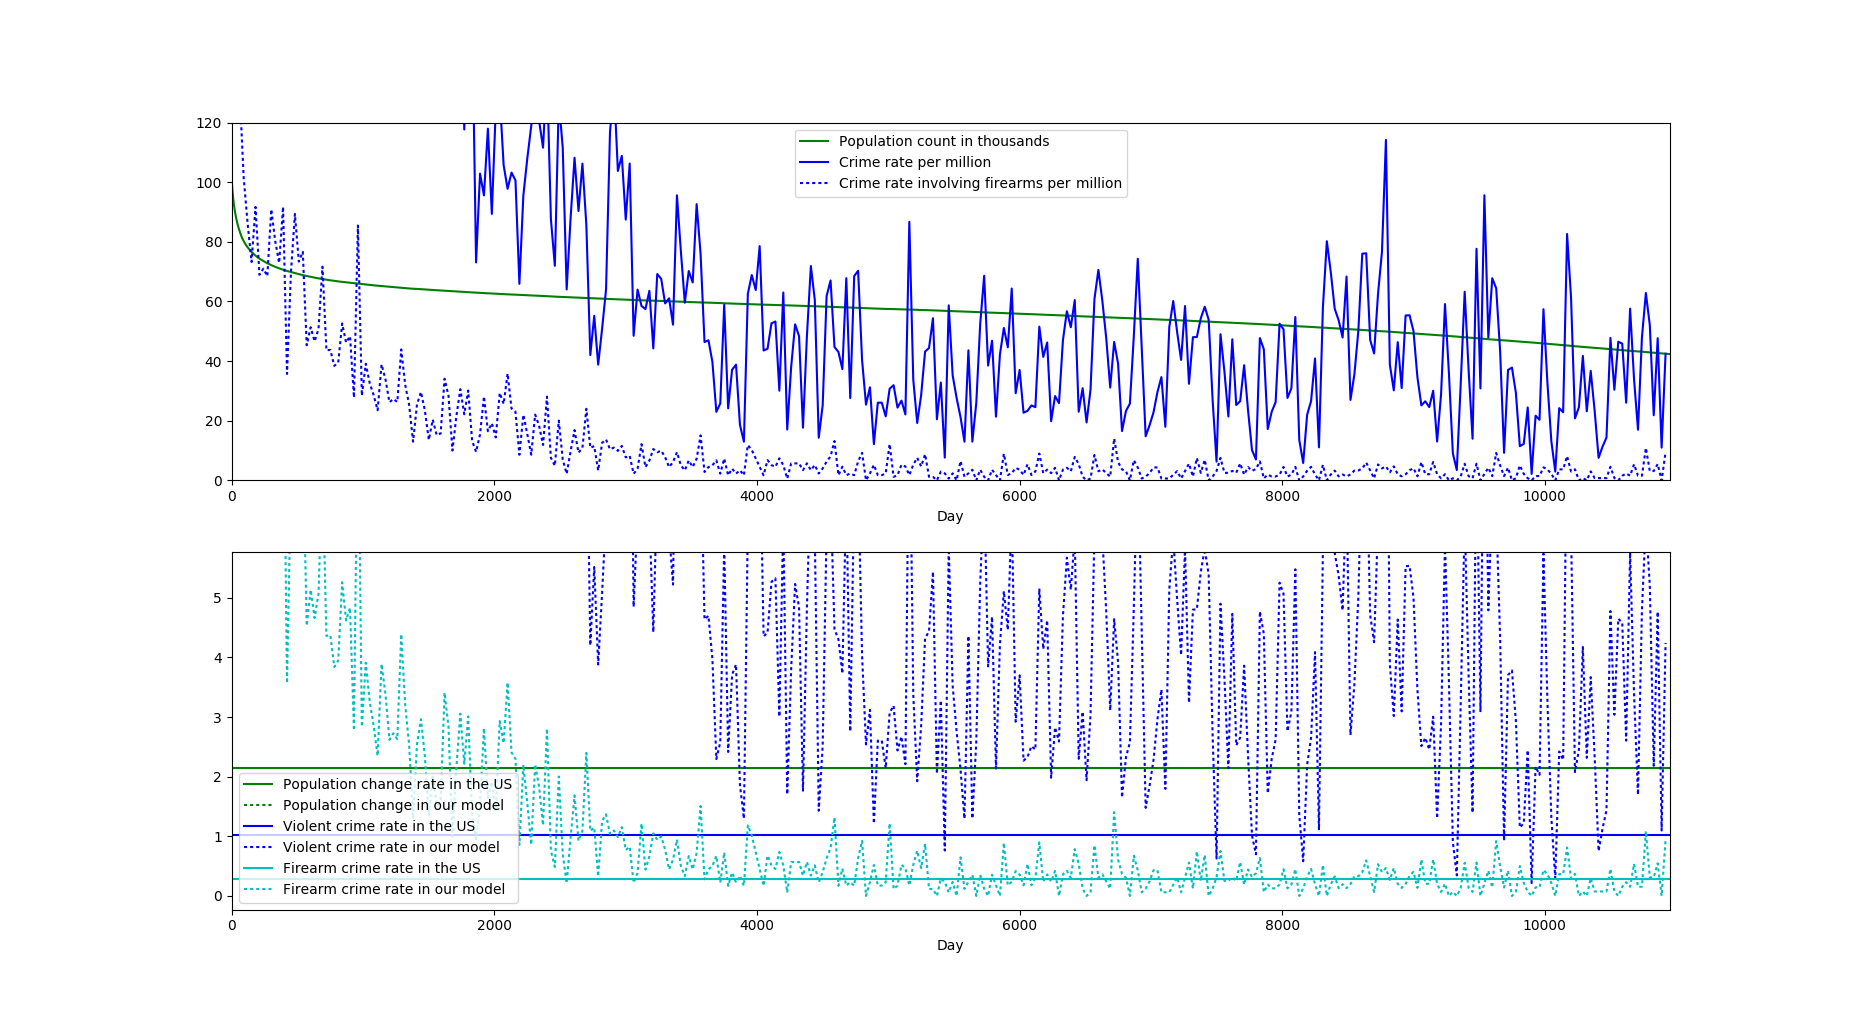
\includegraphics[width=\textwidth]{those_graphs.png}
\caption{Simulation results with chosen parameters}
\label{fig:normal}
\end{figure}

\par
Our first hypothesis was, that imposing increased punishments on violent crime committed while
carrying a gun would decrease violent crime rates. To test this we increased the cost parameter
associated with gun related crimes. The results of the simulation can be seen in figure
\ref{fig:hyp1}. Compared to the run without raised punishment the crime rate in the beginning
of the simulation is lower, while the same for the last two thirds. The gun related crime rate is
significantly lower over the whole course of the simulation.

\begin{figure}[!t]
\centering
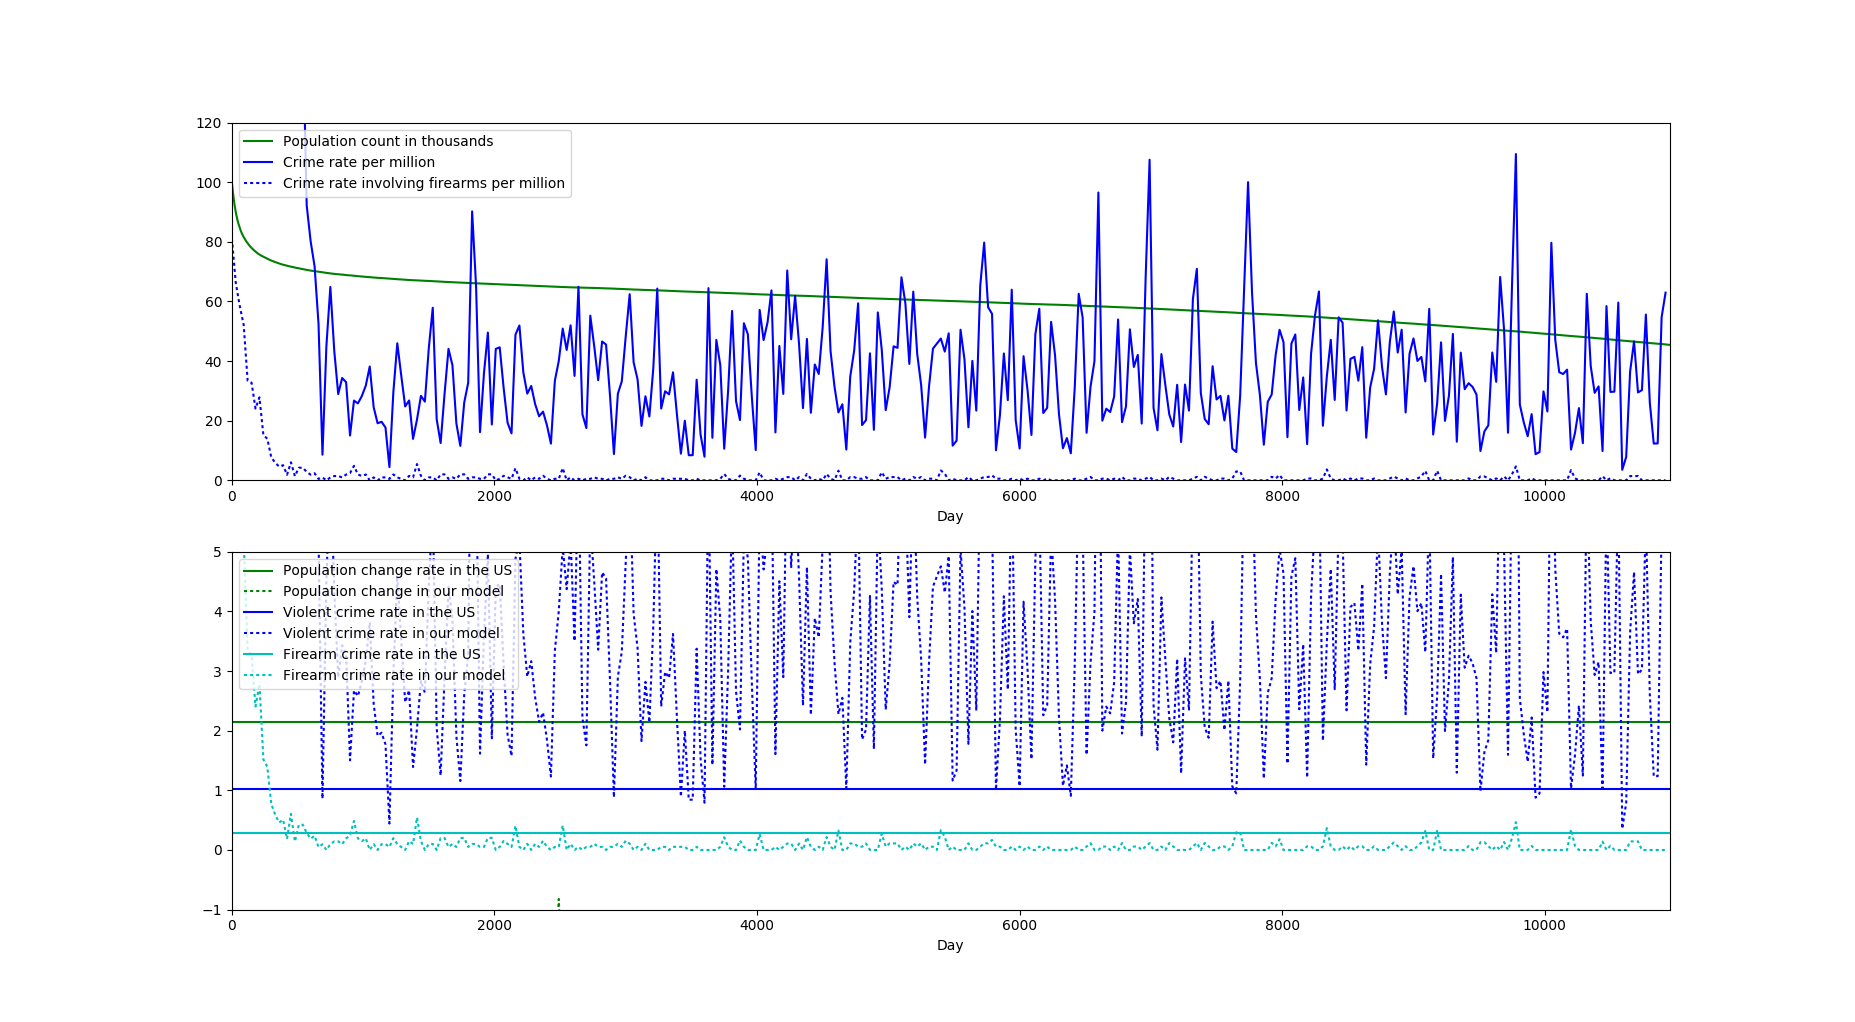
\includegraphics[width=\textwidth]{long_1.png}
\caption{Simulation results with increased punishment}
\label{fig:hyp1}
\end{figure}

\par
Our second hypothesis was, that creating and enforcing stricter rules on gun acquisition and
possession would reduce the rate of violent crime involving firearms. We tested this by removing
guns from any agent who failed to commit a gun related crime, and disallow any agent who has failed
to commit a violent crime from buying a gun, forcing them to acquire one illegally or refrain from
committing the crime. The result of the corresponding simulation can be seen in figure
\ref{fig:hyp2}. Compared to the run without background checks the crime rate is lower, but the
rate of gun related crimes is higher.

\begin{figure}[!t]
\centering
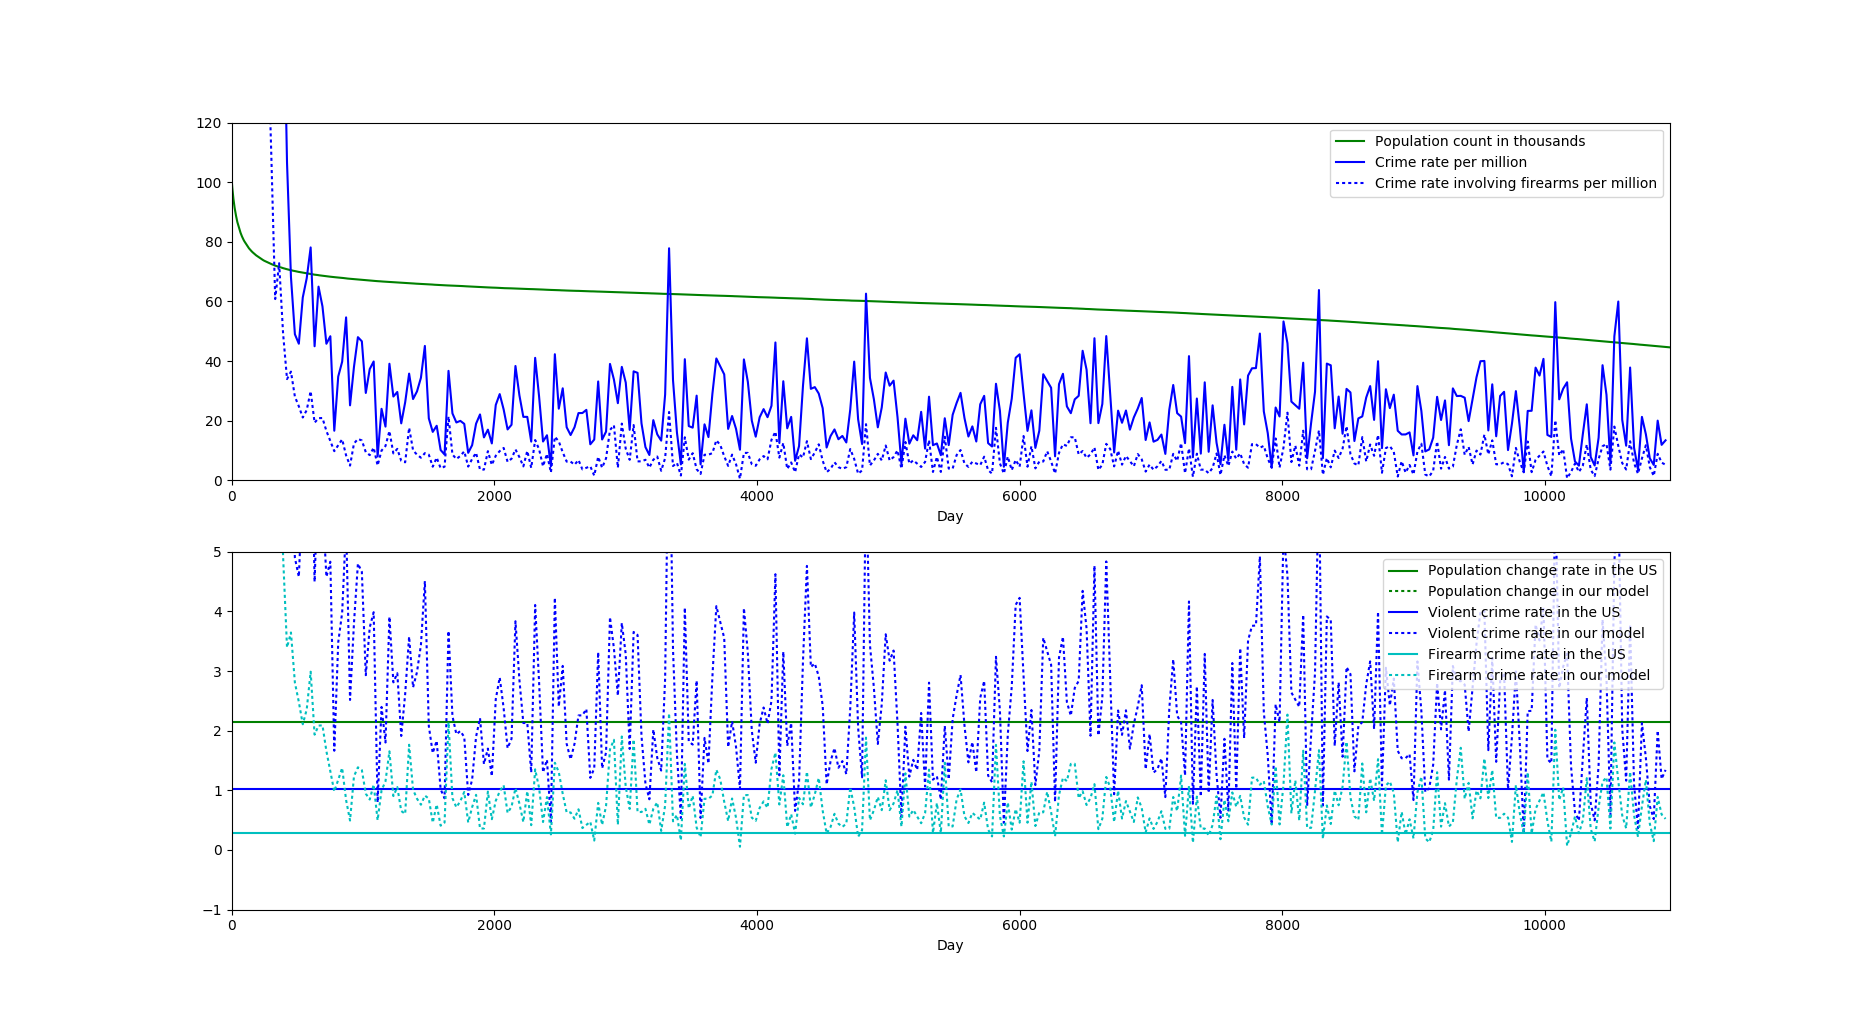
\includegraphics[width=\textwidth]{long_2.png}
\caption{Simulation results with background checks}
\label{fig:hyp2}
\end{figure}

\section{Conclusion}
The simulation output of our model did not exactly match the empirical data. But with good parameters
it came very close and appeared to converge towards the desired value.
This behavior gives a hint that it is possible for our model to be representative for reality.
However to conclude relevant statements, the validity of the model should be examined further with other parameter sets.
The results of our test runs show, that, as far as the model is representative, our hypotheses were largely correct. The lower number of gun related crimes in the first test hints at the crimes being less extensive.

\section{Discussion}
Our model, although relatively complicated, makes a lot of estimates and abstractions and fails
to capture many concepts. It does not include the notion of social groups like families or
friendship circles. Although we included moral propagation and the age based weakening of this
effect as a learning heuristic, there is much more that can be done to improve agent learning,
like agent memory and the perception of behaviors of agents in their social environment. Our model
also does not have a spacial aspect, and thus fails to capture simple constraints on crime execution
like spatial proximity of delinquent and victim, or absence of law enforcement.
Our model changes the emotional state of agents on interactions with other agents. These changes
only represent a small and simplified subset of temperament changes possible in the real world
and don't consider the agent's subjective perception of the event or his situation. The specific
decision making in this model is based on theories grounded in empirical research, but is not
grounded in solid empirical evidence in this specific combination and context.

To handle the complexity of the model was our main issue. Even with a lot of abstractions, the model is still very complicated and therefore it is a hard task to find good parameters. This complexity could be handled in several ways:
\begin{itemize*}
	\item Introduction of more abstractions\\
    This would make the search space for parameters smaller and therefore it would be easier to validate the model.
    \item Gaining empirical basis from surveys\\
    A possibility would be to make surveys to gain an empirical basis for some current parameters.
    Empirical values for some initial distributions could discard a lot of parameters and would have the same effect as the previous option.
    \item Other techniques for parameter search\\
    The automation of the parameter search could be improved with other techniques.
    An idea would be to look at the error output in a numerical way.
    In this area several techniques to minimize the error would be possible to be examined.
    Examples for such methods include the secant method over every dimension and gradient descent.
    For the latter the deviation of the error must be estimated.
\end{itemize*}

Performance optimization is a very crucial task for the validation of the model. The automated parameter search depends on an error computation which requires a simulation of the full ABM. We already put a lot of effort into this area, mostly time complexity related. A new datastructure was designed for our specific requirement of a hashtable which can efficiently output random values that it contains and still have amortized constant insert, remove and access methods.
Further improvements could be made in terms of parallel execution and cache level optimizations.

For performance reasons we used a death distribution that only roughly represented empirical data (see \ref{birthdeath}). But still we used an age distribution during initialization, that fitted empirical data better. This made our model to adapt the age distribution of the agents according to our simplified death distribution, leading to a huge death rate in the first days.
This gave us problems in the parameter search, because the computed error was for one simulation very large because of the big difference of the population change rate from the simulation to the empirical population change rate.
This problem could be avoided, if the age distribution of the model fits to the simplified death distribution. An approach for this would be to simulate only death and birth of agents for a long enough period of time (e.g. 100 years) and use the resulting age distribution for initialization.

% MAIN TEXT

% Place the main text here. Please use only \section, \subsection, and \subsubsection sectioning commands to structure your text. Do NOT use lower sectioning commands, including \paragraph and \subparagraph

%For bulleted, numbered and description lists the class provides three asterisked environments to replace the standard LaTeX ones: itemize*, enumerate*, and description*. Please use these ones as the standard environment may cause issues with the paragraph numbering system.

%\begin{itemize*}
%     \item
%     \item
%     \item
% \end{itemize*}

% hyperlinks (to models, videos, etc.) can be included via the \href command (remember to put \usepackage{hyperref} in the preamble). Check the hyperref documentation for details

%%%%%%%%%%%%%%%%%%%%%%%%%%%%%%%%%%%%%%%%%%%%%%

% FIGURES AND TABLES

% Figures should be placed in the desired position within the text. Please follow the template below.
% Figure widths can be set using absolute dimensions (e.g., [width = 12cm]) or relative ones (e.g., [width = 0.8/textwidth]). We strongly suggest to use the latter option, as this allows automatic adaptation to different paper widths

%\begin{figure}[!t]
%\centering
%\includegraphics[width=????\textwidth]{????}
%\caption{}
%\label{fig:????}
%\end{figure}

% Tables should be placed in the desired position within the text. Please follow the template below

%\begin{table}[!t]
%	\centering
%	\begin{tabular}{????}
%	\toprule
% 	% first line
%	\midrule
%	% tale body
%	\bottomrule
%	\end{tabular}
%	\caption{}
%	\label{tab:????}
%\end{table}

%%%%%%%%%%%%%%%%%%%%%%%%%%%%%%%%%%%%%%%%%%%%%%
% End of  paragraph numbering. Please leave this untouched
\endparano

%%%%%%%%%%%%%%%%%%%%%%%%%%%%%%%%%%%%%%%%%%%%%%

%%%%%%%%%%%%%%%%%%%%%%%%%%%%%%%%%%%%%%%%%%%%%%

% APPENDICES
% Put your appendices here. Please use the normal sectioning command, e.g.,
% \section{Appendix A: <title of the appendix>}
% \section{Appendix B: <title of the appendix>}
% ...

%%%%%%%%%%%%%%%%%%%%%%%%%%%%%%%%%%%%%%%%%%%%%%

% ENDNOTES. Please uncomment the line below in case of notes.
% \theendnotes

%%%%%%%%%%%%%%%%%%%%%%%%%%%%%%%%%%%%%%%%%%%%%%

% REFERENCES.
% The JASSS bibliographic style file (jasss.bst) is included in the bundle. Please use BibTeX, not BibLaTeX.
% Use natbib commands for references (\citep{}, \citet{}, etc.), not standard LaTeX ones (\cite{}).
% Remember to include the doi and url fields in your bib database. The address field should be included for books.
% Please upload the bib file (not just the bbl one) when submitting.

\bibliographystyle{jasss}
\bibliography{references}{} % Please set the right name for your bib file

%%%%%%%%%%%%%%%%%%%%%%%%%%%%%%%%%%%%%%%%%%%%%%

\end{document}